\chapter{Implementation-2}
\label{ch:implementation2}
\section*{Part 2}
\label{sec:part2}
In the part 1, we tried implementing vid\_orbslam3 node to perform VI-SLAM on our drone setup. As explained in the previous chapter, the attempts failed to give results for various reasons. To continue the pose and keyframe trajectory estimation, we planned to use GPS data with Visual SLAM and adapt it to a local coordinate system of choice. This chapter explains the method, architecture, challenges, observations and results of the implementation.

\section{Architecture}
\label{sec:architecture2}
The architecture is a continuation of the previous architecture from Section \ref{fig:architecture}. The gps\_process node is a stand-alone node which runs on a local PC subscribing to the keyframe graph topic from the vid\_orbslam3 node and the GPS topic from the drone. The following block diagram depicts the architecture of the implementation.

\begin{figure}[h]
    \centering
    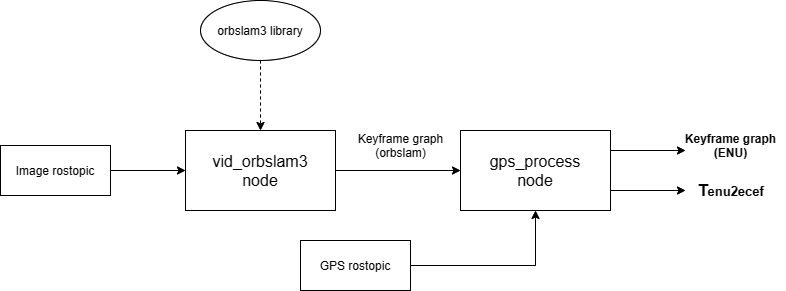
\includegraphics[height=4.5cm, width=10cm]{Images/archi2.png}
    \caption{Architecture for Visual Inertial SLAM with GPS}
    \label{fig:archi2blk}
\end{figure}

A suitable method is used to estimate the keyframe graph in East-North-Up (ENU) system and a static transform is published between ENU and Earth Centric Earth Fixed (ECEF) system for external tool or software for visualization. There are other approaches to fuse gps data into the bundle adjustment of the SLAM system, but it would become a separate project to develop. Finally it was decided to move ahead with our architecture.

\section{Processing Keyframe graph}
\label{sec:processingKFgraph}
The vid\_orbslam3 node was reverted back to work as Visual SLAM mode. To transform the keyframe graph generated by ORBSLAM3 to ENU system, the whole set of keyframe list had to be published as and when a new keyframe is added to the list. The native ORBSLAM3 library has an entity called Atlas that stores all the keyframes at the current instance. When loop closure occurs or redundant frames are removed, Atlas updates itself with a freshly updated keyframe list. We make use of this in our node by adding a new method to the native library. The method is called \emph{System::getAtlas} and it returns pointer to the current Atlas. We recomplied the library and invoked this method in the vid\_orbslam3 node.\\

For every image frame that is subscribed, a fresh list of keyframe graph is updated in vid\_orbslam3 node. For every new keyframe graph obtained it is then published as a rostopic named as /KeyframeGraphSLAM. This topic is of the message type vid\_orbslam3::KeyframeGraph, which is a custom rosmessage that was that was created by us to hold all the current keyframes in an array.\\

Now moving on, we started developing gps\_process node inside our development package. The gps\_process node needs two inputs to process: /KeyframeGraphSLAM, which gives the whole KeyframeGraph at the current instance and the GPS topic /dji\_osdk\_ros/gps, which gives current GPS location of the drone in WGS84 system. Using these two, the whole KeyframeGraph in SLAM co-ordinate system can be converted into East-North-Up (ENU) co-ordinate system. In the further sections we shall explain how the transformation is performed to achieve the task.

\section{Approach to estimate T\textsubscript{slam2enu}}
\label{sec:approachTslam2enu}
The gps\_process node subscribes to keyframe graph topic and gps topic for the estimation purpose. The lift off of the drone is set as the initial coordinate for the purpose of ENU reference. All the gps messages are stored in a list for gps stamping the keyframe. The first step in this approach is to gps stamp every frame in the keyframe graph. Every keyframe in the graph is sorted using the timestamp of the gps message. Since there might be a slight delay in milli-seconds between the KeyframeGraph topic and gps topic, a time difference of less than 2 ms is allowed. By doing this, all the keyframes in the KF graph are tagged with respective gps location in WGS84 format and ENU format. To convert gps location to ENU format, we used GeographicLib \cite{GeographicLib} which offers WGS84 to ENU and WGS84 to ECEF conversions. These tagged keyframes are stored into a list with elements formated as a custom data structure containing pose, gps location and ENU point information.\\

\begin{lstlisting}[language=bash, basicstyle=\small]
struct GPSKeyframe {
 tf::Vector3 ENU;  
 sensor_msgs::NavSatFix gpsCoord; 
 vid_orbslam3::KeyframeStamped KF; 
};
\end{lstlisting}

Further, the stored list is iterated over for SLAM positions in keyframes and ENU positions are separated into separate list for the estimation process. The main idea is to obtain a transformation between the SLAM coordinate system and ENU coordinate system. We make use of colmap's \cite{schoenberger2016sfm} similarity transform and a method was developed in gps\_process node to estimate the transformation. The method requires 2 lists with different coordinate systems.For every new callback from the ros node, a new transformation matrix  T\textsubscript{slam2enu} was estimated. Using this, all the keyframes or poses in the stored list was transformed to ENU coordinate system. Further, a posearray was created and published as a topic named /KeyframeGraphENU.\\

Visualization of the above published topic resulted in an oblique trajectory. The drone flew across the area resulting path trajectory plane is parallel to the earth's surface. Theoretically, a similarity transform should correct any such irregularities with the input to a referenced coordinate system. After multiple attempts to correct this, we analysed the input trajectory and tested the same estimation strategy using 2 static data files, one containing SLAM points and corresponding ENU points. 

\section{Observation in static file data analysis}
\label{sec:staticapproach}
The Visual SLAM generated keyframe trajectory and corresponding ENU points were saved into two different files. As observed from the previous section, the keyframe trajectory in ENU was oblique with respect to the surface of the earth. The input trajectory file generated by SLAM system was plotted to check the sanity of the results from ORBSLAM3. The input /KeyframeGraphSLAM to the gps\_process node was itself oblique as shown below.

\begin{figure}[h]
    \centering
    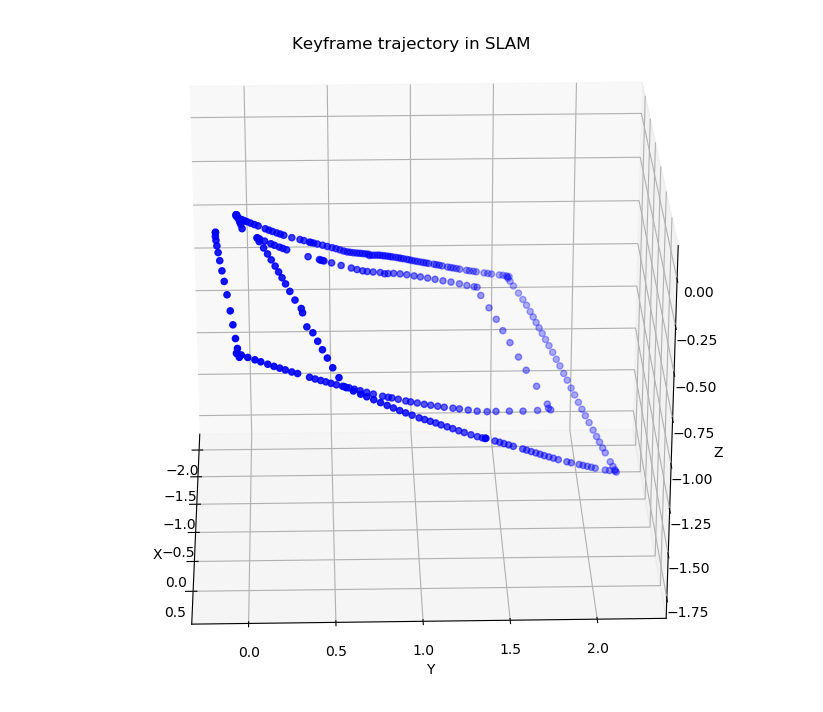
\includegraphics[height=11cm, width=15cm]{Images/KFTrajectoryinSLAMFront.png}
    \caption{Keyframe trajectory in SLAM, Front view}
    \label{fig:kfgraphSLAMfront}
\end{figure}

\begin{figure}[h]
    \centering
    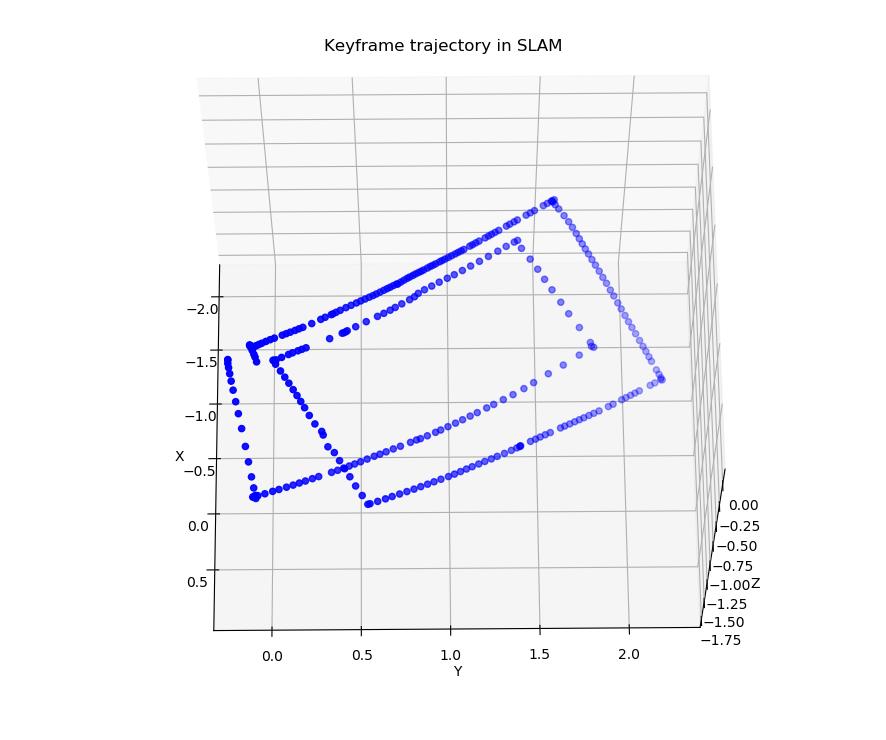
\includegraphics[height=11cm, width=15cm]{Images/KFTrajectorySLAMTop.png}
    \caption{Keyframe trajectory in SLAM, Top view}
    \label{fig:kfgraphSLAMtop}
\end{figure}

From the top view \ref{fig:kfgraphSLAMtop}, it looks to be flat and parallel to the surface. But when observed from the front \ref{fig:kfgraphSLAMfront} we can clearly see the oblique nature of the result. Naturally, when all the current keyframes on list is considered for transformation the resultant in the ENU coordinate system also produces an oblique trajectory curve. This is due to the cumulative effect that Visual SLAM produces from scale ambiguity.\\ 

VI-SLAM would have corrected this obliqueness using it's Inertial sensors (IMU). Since we are not using VI-SLAM, a different approach is needed to tackle overcome this. The measurement scale in the figure \ref{fig:kfgraphSLAMfront} and \ref{fig:kfgraphSLAMtop} are in orbslam3 scale. Usually, this found to be normalized internal SLAM system.

\section{Windowed-selection approach and Robust alignment}
\label{sec:windowandrobust}
Instead of considering all the points in SLAM and ENU system for estimating Transformation matrix, we can construct a window of N where N = 3, 5, 7, 11. This window can slide over both the lists (SLAM points and ENU points), select a group of N elements in the range. For this bunch of N elements are used for estimating transformation matrix. The obtained transformation matrix is used to transform the middle element in the SLAM points window and further the transformed point is added onto the list of transformed points. This process was performed for the complete set of points using both files. When the resultant list of converted points were plotted, we found that the obliqueness of the trajectory was solved. We chose to use window size N = 3. Although, we tried for all the above mentioned sizes.

\begin{figure}[h]
    \centering
    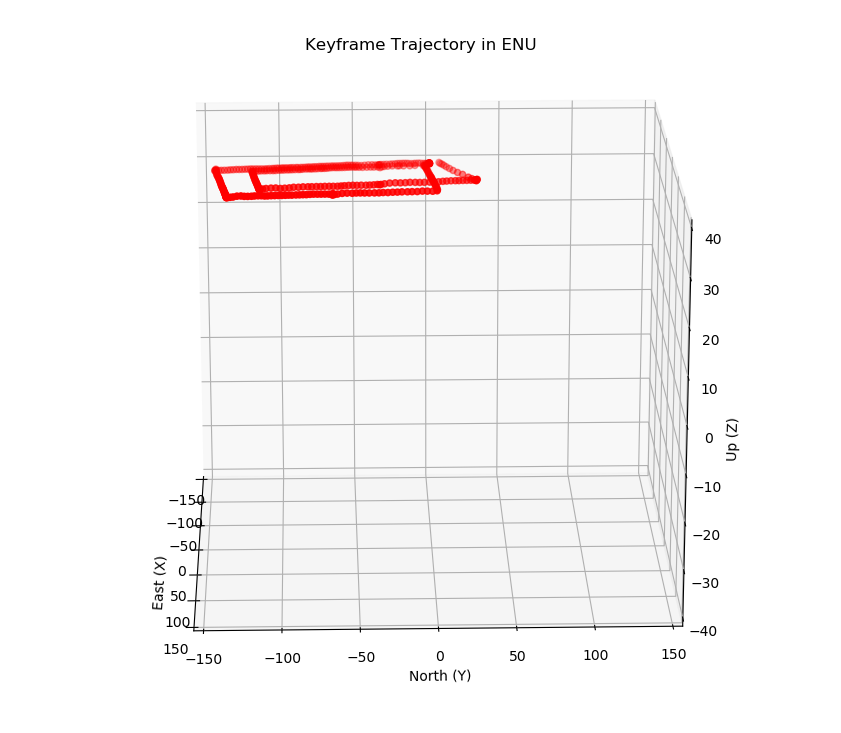
\includegraphics[height=11cm, width=15cm]{Images/KFTrajectoryENUwindowedFront.png}
    \caption{Point trajectory in ENU using window approach, Front view}
    \label{fig:kfgraphENUfront}
\end{figure}

\begin{figure}[h]
    \centering
    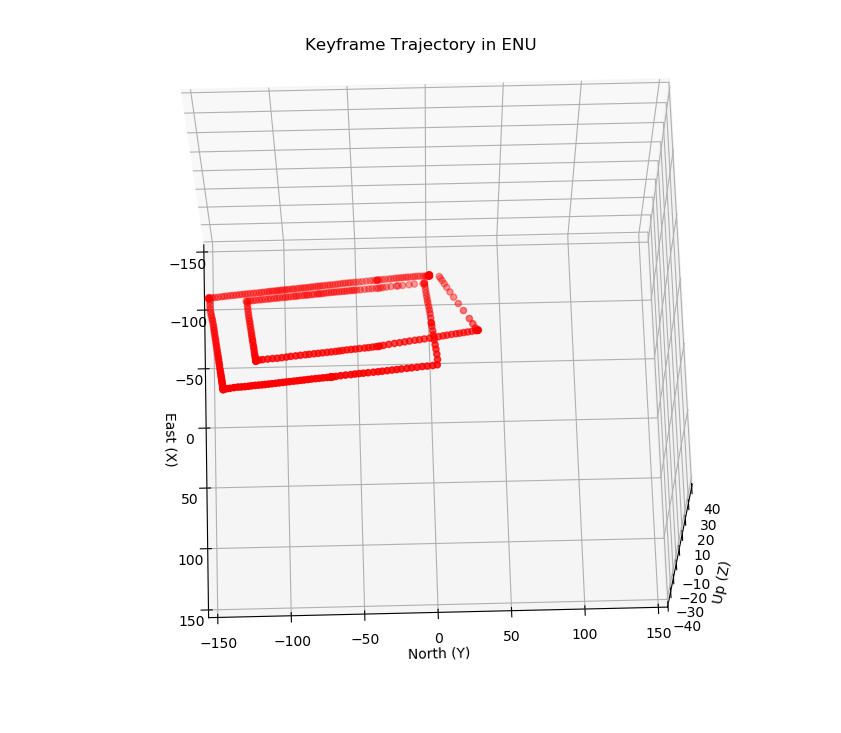
\includegraphics[height=12cm, width=15cm]{Images/KFTrajectoryENUwindowedTop.png}
    \caption{Point trajectory in ENU using window approach, Top view}
    \label{fig:kfgraphENUtop}
\end{figure}

Though initially, a disjoint set was selected from the list of elements by the window. This would omit 2 out of 3 elements from the selected scope and convert only the middle element. Later on, an overlapping window was used to select the window of elements resulting in full usage of all the points except couple of initial points which we were least interested in. The figures \ref{fig:kfgraphENUfront} and \ref{fig:kfgraphENUtop} are the results of an overlapping window approach and the scale is in meter (m).\\

Normal similarity transform method from colmap is enough to get a good transformation matrix estimation. But when we tested for multiple attempts, the estimation was not as expected. One of the cases where couple of points were estimated above the trajectory plane. For a real-time implementation like in our case, a more rigid estimation is required. Colmap also comes with a method that estimates transformation matrix using similarity transform with robust alignment.\\

Robust alignment uses RANSAC parameters to fit the closest and meaningful outcome for the transformation matrix. This helps in estimating the trajectory points more accurately and closer to actual point in real world scenario. The robust alignment addition was made in our static file data analysis and was tested on the same set of files for sanity. The similarity transform method in our gps\_process node was later on adapted to robust alignment.  

\section{Windowed approach for real-time processing}
\label{sec:windowapproachrealtime}
The real-time processing of the topics using the ros nodes vid\_orbslam3 and the gps\_process would yield the expected results and will prove the sanity of our approach discussed in the previous section. The overlapping windowed approach with robust alignment was added and adapted into our gps\_process node. For the real-time scenario, we do not have pre-defined points or keyframes in hand to slide over the whole set. The approach had to be modified to select the last N elements from the keyframe graph list and the ENU points list for the purpose of estimation of transformation matrix. N denotes the size of the window. The keyframes in the SLAM list were converted to ENU system and added onto a new list of keyframes. New keyframes to this list were added only when a new keyframe was available at the input /KeyframeGraphSLAM topic to avoid duplicate keyframes in the list. Further, the list of keyframes were published as a ros::PoseArray for further usage.\\

A static transform between ENU and ECEF (T\textsubscript{enu2ecef}) was also calculated using the initial ENU point after the lift off and was eventually published as a broadcast. This transform can be used by third-party tools and software to visualize the drone and camera poses on an earth-like environment by converting keyframe graph in ENU to earth scale.

\newpage

\section{Results}
\label{sec:results}
A simulation was executed using our nodes with recorded rosbag where the entire behaviour of the drone was captured. The following snapshots are the results of our implementation.

\begin{figure}[h]
    \centering
    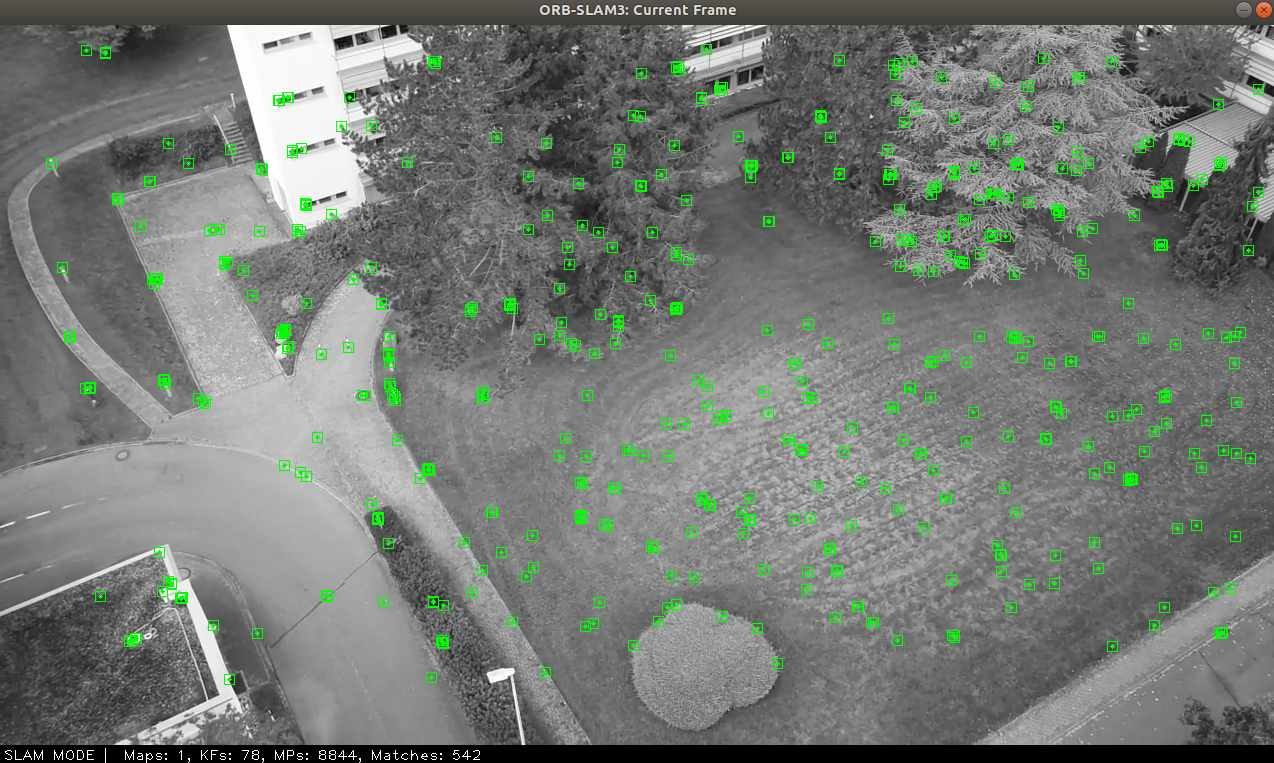
\includegraphics[height=6cm, width=12cm]{Images/camera_frame_orbslam3.png}
    \caption{Camera frame from orbslam3 visualization window.}
    \label{fig:cameraframe}
\end{figure}

\begin{figure}[h]
    \centering
    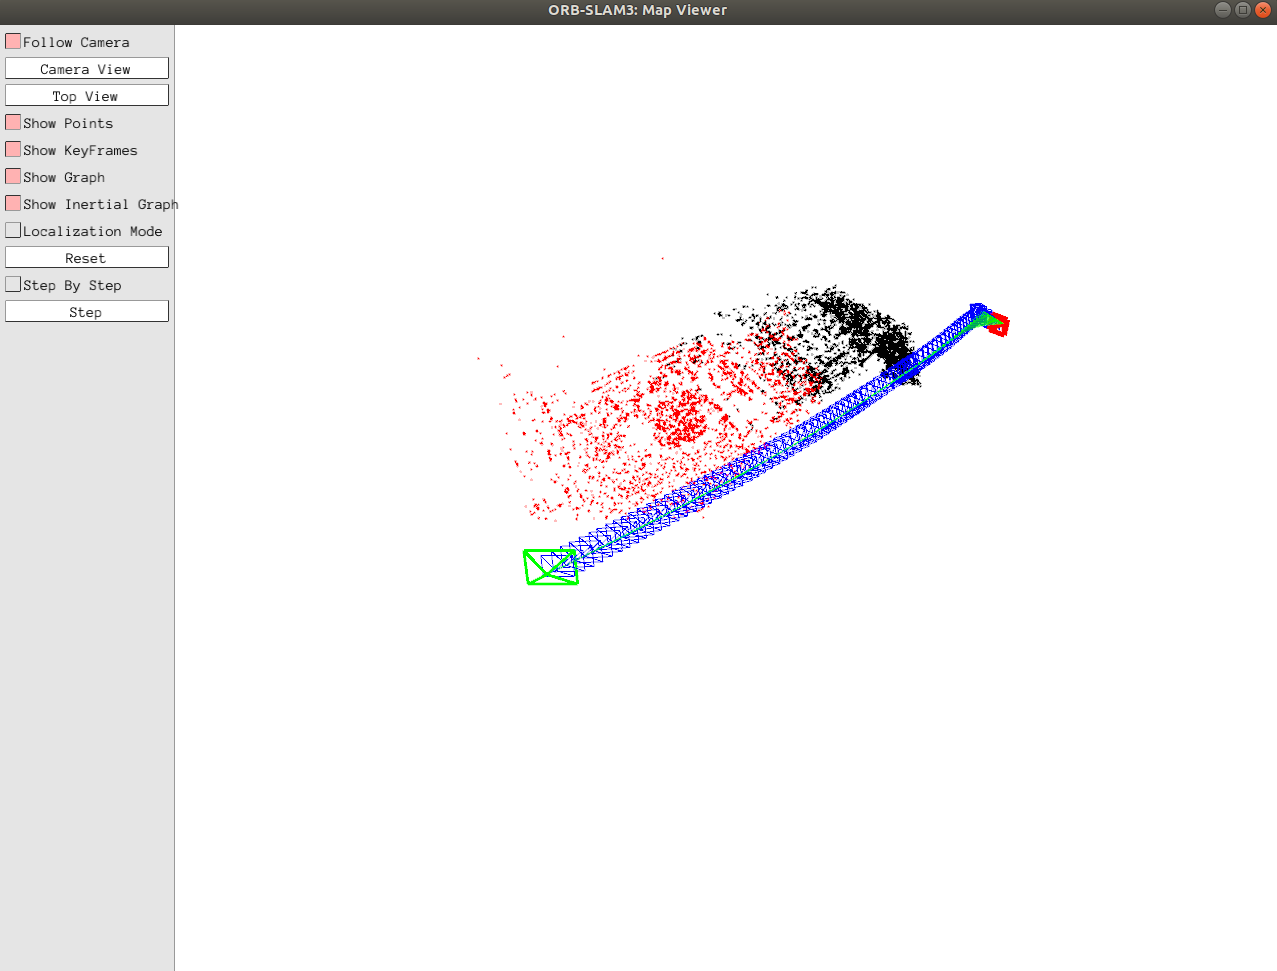
\includegraphics[height=6cm, width=12cm]{Images/trajectory_orbslam3.png}
    \caption{Keyframe trajectory atlas from orbslam3 visualization window.}
    \label{fig:kftrajatlas}
\end{figure}

The above figures \ref{fig:cameraframe} and \ref{fig:kftrajatlas} are the snapshots of the camera frame containing key points detected and the keyframe trajectory atlas depicting the current camera pose at a given instance of time. 

\begin{figure}[h]
    \centering
    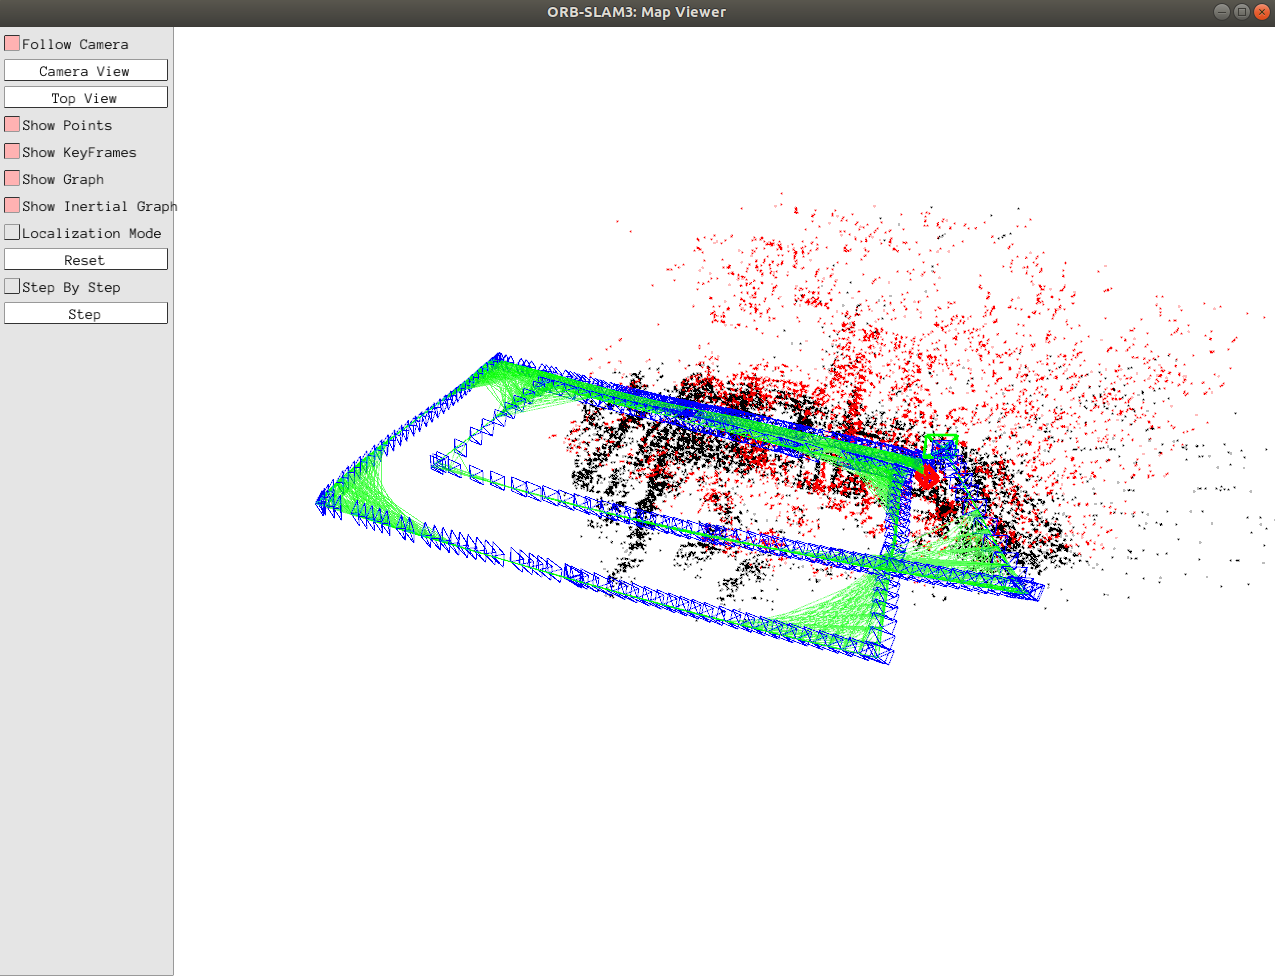
\includegraphics[height=6cm, width=12cm]{Images/trajectory_final_orbslam3.png}
    \caption{Complete Keyframe trajectory atlas from orbslam3 visualization window.}
    \label{fig:kftrajatlascomplete}
\end{figure}

The above figure \ref{fig:kftrajatlascomplete} shows the complete keyframe trajectory with the starting camera pose (red rectangle), detected key points, repeated key points and loop closure. The estimation of the above Visual SLAM depiction in ENU coordinate system resulting in a point trajectory is as shown in the following figures.

\begin{figure}[hbt!]
    \centering
    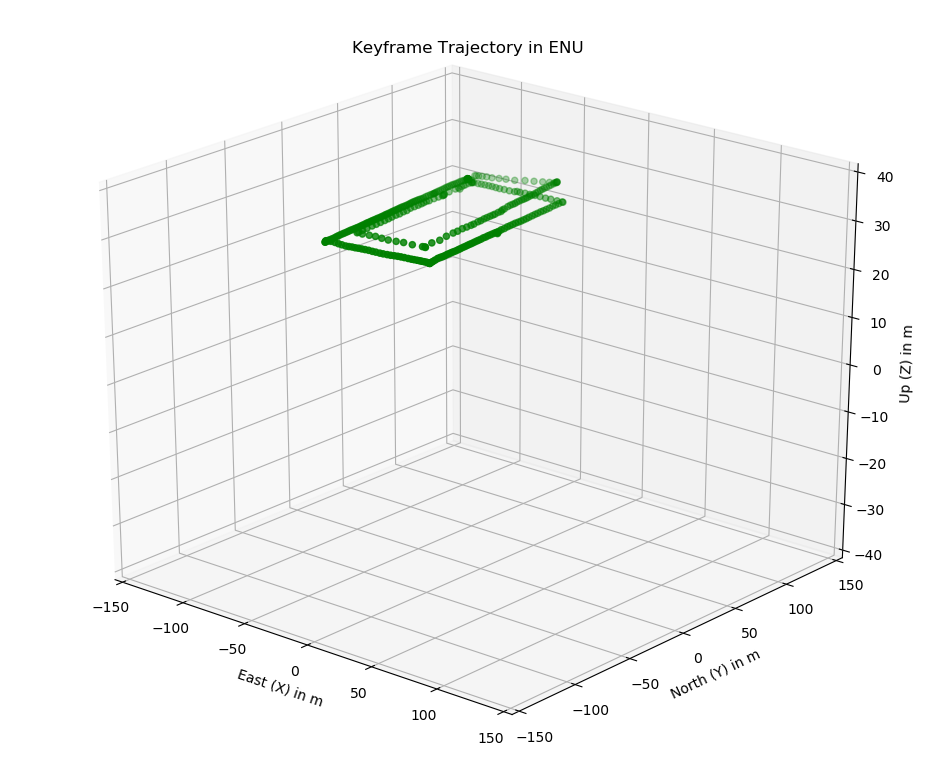
\includegraphics[height=9cm, width=13cm]{Images/kftrajectoryENUFinalIsometric.png}
    \caption{Point trajectory in ENU, Isometric view}
    \label{fig:kfgraphENUIsofinal}
\end{figure}

\begin{figure}[hbt!]
    \centering
    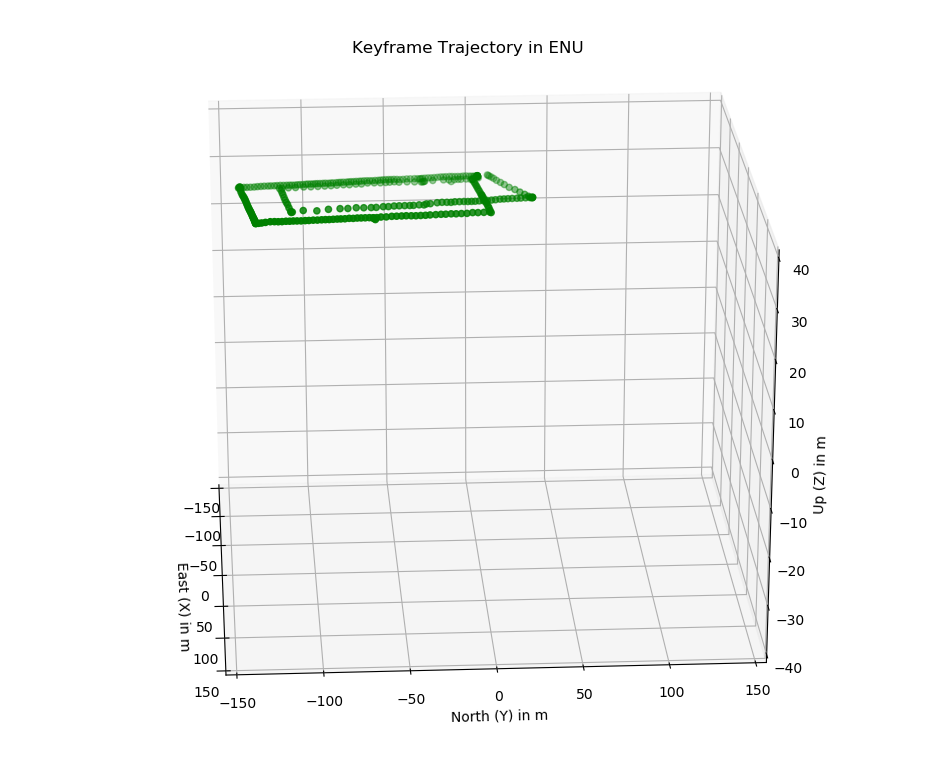
\includegraphics[height=9cm, width=13cm]{Images/kftrajectoryENUfinalFront.png}
    \caption{Point trajectory in ENU, Front view}
    \label{fig:kfgraphENUfrontfinal}
    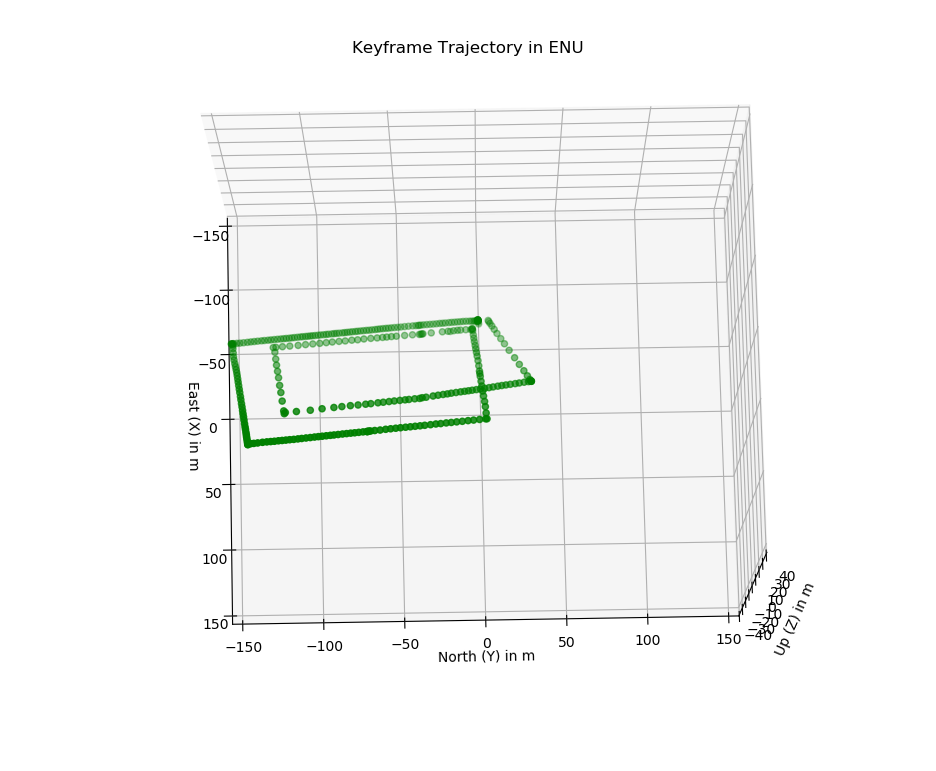
\includegraphics[height=9cm, width=13cm]{Images/kftrajectoryENUfinalTop.png}
    \caption{Point trajectory in ENU, Top view}
    \label{fig:kfgraphENUTopfinal}
\end{figure}

\newpage
We can clearly see the height of the flight at around 40 m above the grond in the Front view figure \ref{fig:kfgraphENUfrontfinal} which is the same height at which the drone flew. Even though the task is called as "Keyframe trajectory" estimation, the orientation visualization of the camera was not possible due to unknown issues with the format. An approach to correct this issue was planned but due to shortage of time duration in my internship the work was halted till this stage.

\section*{Additional task}
\section{Stereo rectification ROS node}
\label{sec:stereorectinode}
DJI Matrice 210 v2 RTK drone has stereo camera and provides many features in-built like disparity map, filtered disparity map and point cloud and also rectified image stream. Stereo rectification from the advanced sensing application of the drone requires CUDA support. Even though Manifold 2 supports CUDA, installing the DJI SDK and ROS SDK with CUDA dependency would drive the already hanging overhead to extreme level. \\

\begin{figure}[h]
    \centering
    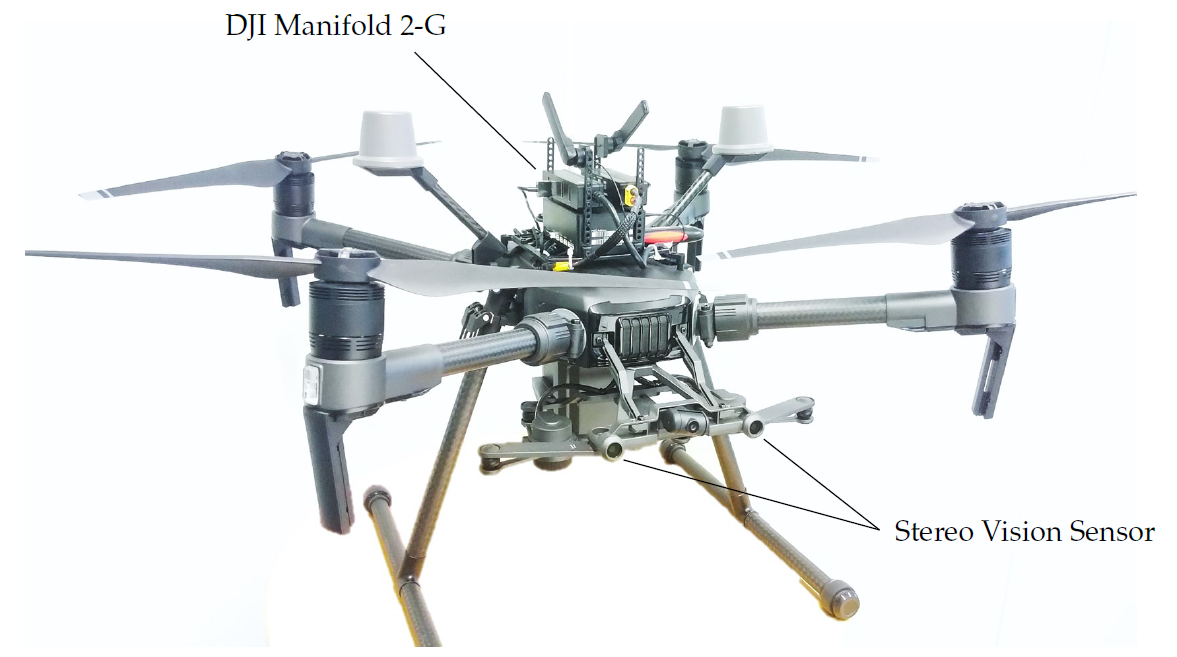
\includegraphics[width=11cm,height=7cm]{Images/djidronewithstereo.PNG}
    \caption{DJI Matrice 210 v2 RTK with integrated stereo vision sensor. Source: Mr Boitumelo Ruf}
    \label{fig:dronestereo}
\end{figure}

We wanted to develop a separate stand-alone node for the stereo image rectification. A ROS package named vid\_rectify \cite{vid_rectify} was developed to rectify the stereo images from the drone. The stereo cameras of the drone were calibrated and the stereo intrinsic parameter file was generated in OpenCV \cite{opencv_library} standard format. The node was tested and used in a project named "Real-time SGM Stereo Optimized for
Embedded ARM and CUDA Devices Mounted on Low-cost UAVs" authored by Mr Boitumelo Ruf and team. For an input rate of 20 fps, we obtained 20 fps output without any loss or frame drops in the process. The package is generic and compatible on any stereo setup. The documentation and the code base can be found in my github repository \cite{vid_rectify}.
 


